\paragraph{RoboTwin depth-teacher failure case.}
RoboTwin contains visually clean, texture-sparse simulator scenes.  This makes it
a useful stress test for geometry-aware policies that rely on a monocular
foundation model teacher.  In the \texttt{handover\_block} task we therefore
compare the Pi3X teacher cache against simulator ground-truth depth, using the
same camera views and frame indices used by policy training.  Because the
student is trained on the raw Pi3X \texttt{log\_z} targets, we select the
frame with the largest mean absolute log-ratio between the Pi3X median depth and
the simulator-GT median depth across the three cameras.  We also report a
scale-invariant shape error, computed after robustly normalizing each log-depth
map within the frame, to separate global scale mismatch from relative geometry.

Figure~\ref{fig:robotwin-pi3x-worst} shows the automatically selected
example: episode 24, frame 227.  The error is
most severe in the right wrist camera: Pi3X predicts a median
depth of 3.535m while the simulator GT median is
0.027m, a 132.4$\times$
mismatch.  Averaged over the three cameras, the selected frame has mean
absolute log-ratio 3.56 and scale-invariant MAE 0.17.
Thus the auxiliary target is geometrically miscalibrated in the clean simulator
domain even when the RGB image is unambiguous and ground-truth depth is
available.

This explains the negative transfer observed for Pi3X-distilled RoboTwin
policies: the auxiliary target can inject a confident but geometrically wrong
prior in the clean simulator domain.  Replacing the monocular teacher with
simulator ground-truth depth removes this source of target noise, which is why
the GT-only variant improves success rate even though the Pi3X-distilled variant
can have lower training losses.

\begin{figure}[H]
  \centering
  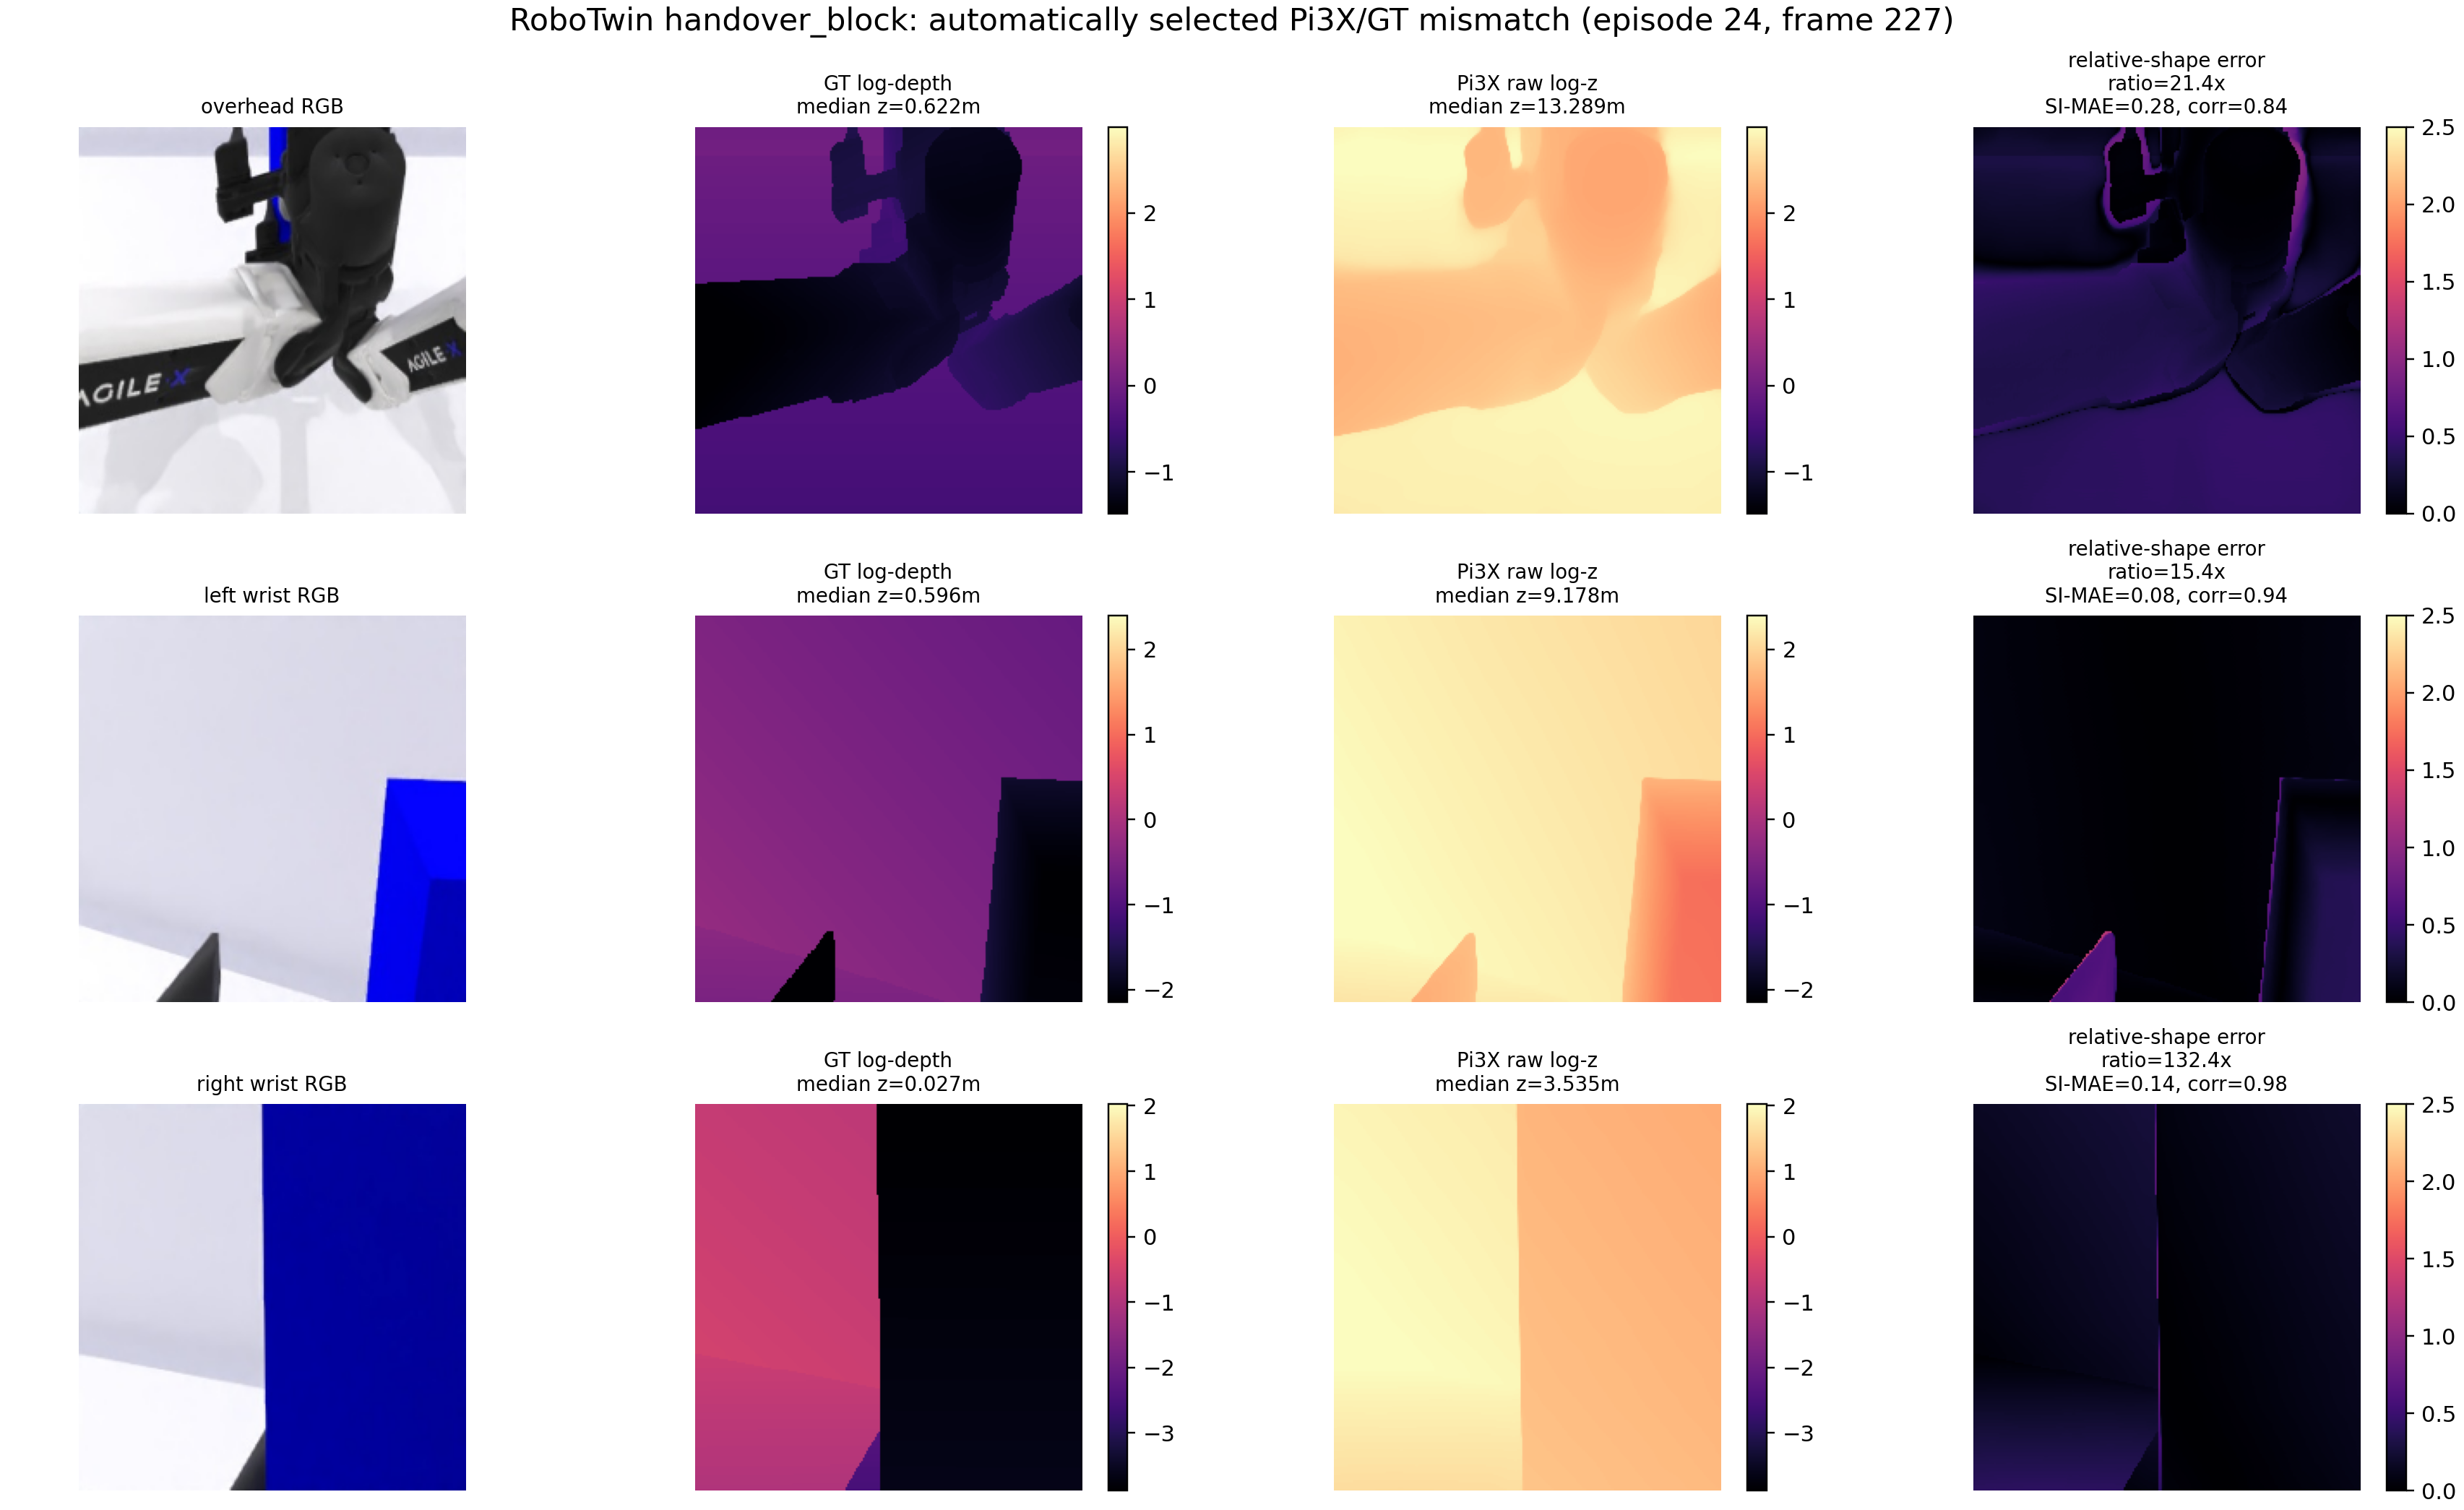
\includegraphics[width=\linewidth]{paper_assets/robotwin_handover_pi3x_appendix/handover_block_pi3x_gt_worst_ep000024_frame0227.png}
  \caption{Worst automatically selected Pi3X/GT depth mismatch in RoboTwin
  \texttt{handover\_block}.  GT and Pi3X log-depth panels use the same color
  scale per view.  The right column shows the remaining relative-shape error
  after per-frame robust log-depth normalization.}
  \label{fig:robotwin-pi3x-worst}
\end{figure}

\begin{figure}[H]
  \centering
  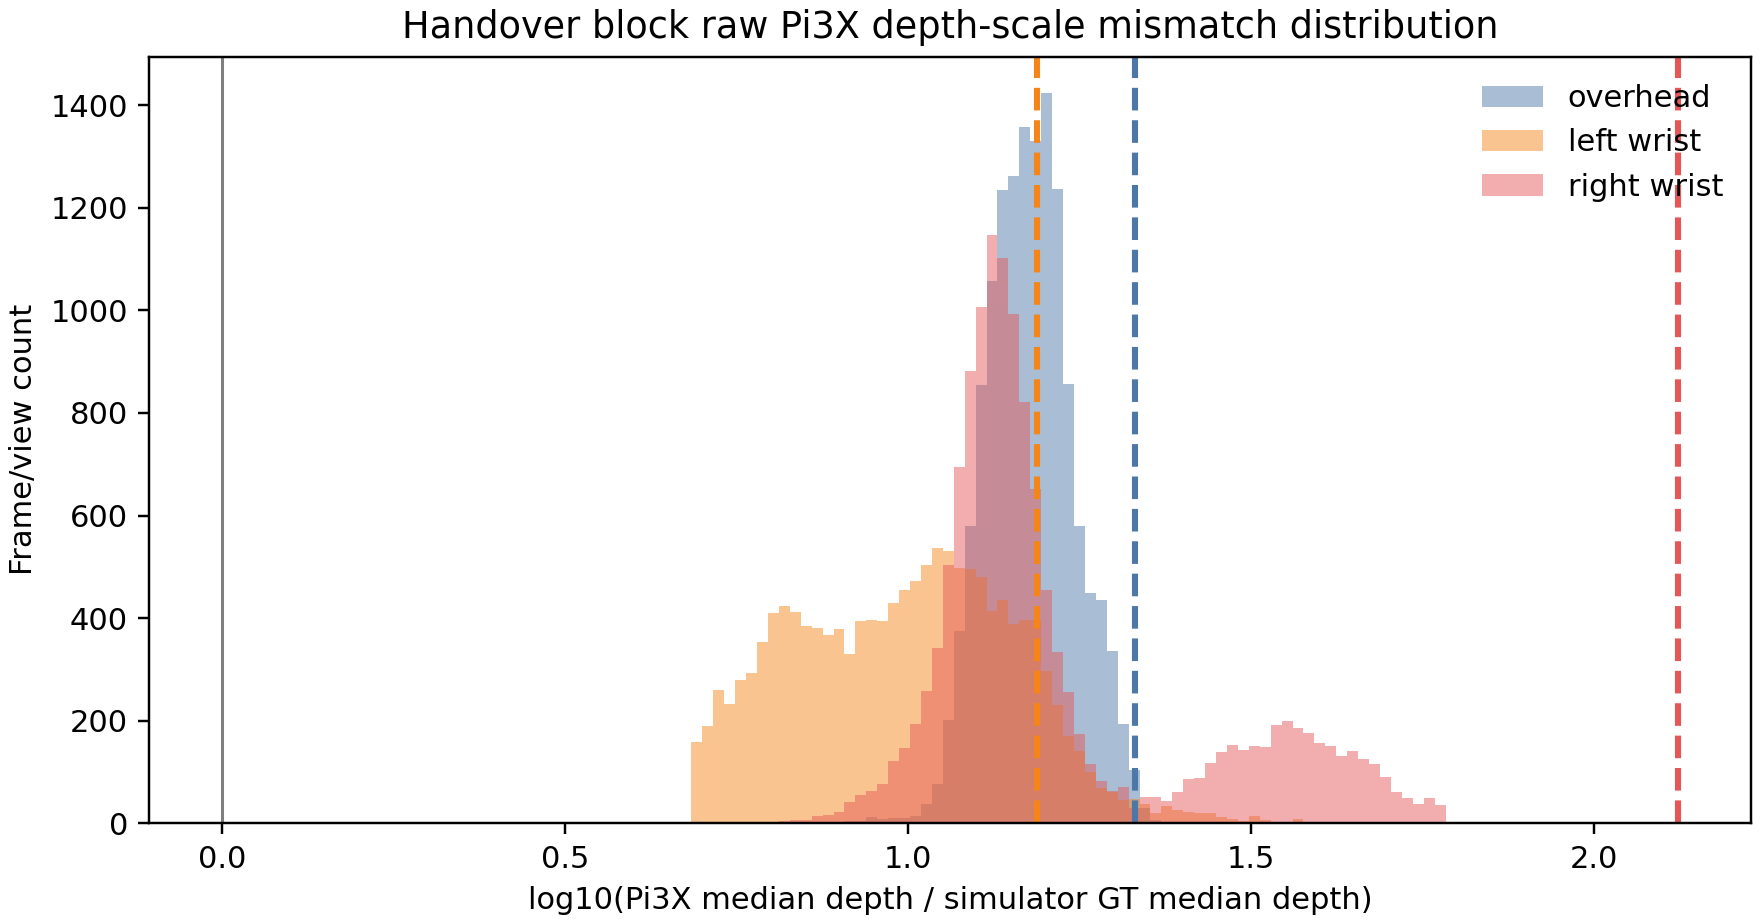
\includegraphics[width=0.72\linewidth]{paper_assets/robotwin_handover_pi3x_appendix/handover_block_pi3x_gt_error_histogram.png}
  \caption{Distribution of raw median-depth scale mismatch across the
  handover-block cache.  Zero means Pi3X and simulator GT have the same median
  depth.  Dashed vertical lines mark the three views in the selected failure
  frame.}
  \label{fig:robotwin-pi3x-error-hist}
\end{figure}
